%% This is an example first chapter.  You should put chapter/appendix that you
%% write into a separate file, and add a line \include{yourfilename} to
%% main.tex, where `yourfilename.tex' is the name of the chapter/appen
dix file.
%% You can process specific files by typing their names in at the 
%% \files=
%% prompt when you run the file main.tex through LaTeX.
\chapter{Partition Function Computation and Improvements}
\section{Introduction}

The partition function for a thermodynamic system of fixed volume, in
contact with a heat reservior with absolute temperature $T$, is
\begin{equation} Z = \sum_s e^{-E(s)/ RT }, \end{equation}
where $s$ denotes a particular state of the system, $E(s)$ is the
energy of that state, and $RT$ is the gas constant multiplied by the
temperature, specified above. Each particular term in the sum is
called that state's Boltzmann factor. The probability of a state is
then said to be its Boltzmann factor divided by the partition
function, or
\begin{equation} P(s) = \frac{1}{Z}e^{-E(s)/RT}.  \end{equation}
In our model an RNA strand is such a thermodynamic system, its
secondary structure is its state, and the rest of the cell is the
reservoir of heat. We assign each secondary structure an energy
according to the free energy model described in Chapter 1. According
to this model, the energy of a secondary structure is the sum of the
energies of its loops. 

To compute the partition function we must sum up every possible
secondary structure. There are many possible secondary structures, on
the order of $1.8^n$ where $n$ is the sequence length. However, the
computation of the partition function benefits greatly from the linear
nature of the energy model: it allows us to recursively define the
partition function. For example, say we have computed the full
partition function of a strand of $n$ bases, define a function $Q$
such that:
\begin{equation}
Q(i, j) = \text { sum of boltzmann factors for every structure contained between } i \text{ and } j.
\end{equation}
The full partition computation can therefore be represented as the
function $Q$ acting on the bounding two bases $1$ and $n$: 
\begin{equation}
 Q(1, n) = \sum_{s \text{ on } [1,n]} e^{-E(s)/RT}.
\end{equation}
If we now extend the strand by attaching a small hairpin to the end,
as pictured in Figure \ref{fig:attachedHairpin}, there is no need to
go back and recompute the energy of every single secondary structure,
rather we can just multiply the already-computed partition function by
the boltzmann factor of the hairpin turn (let $E(h)$ be the hairpin
energy) to get the new partition function:
\begin{figure}[h]
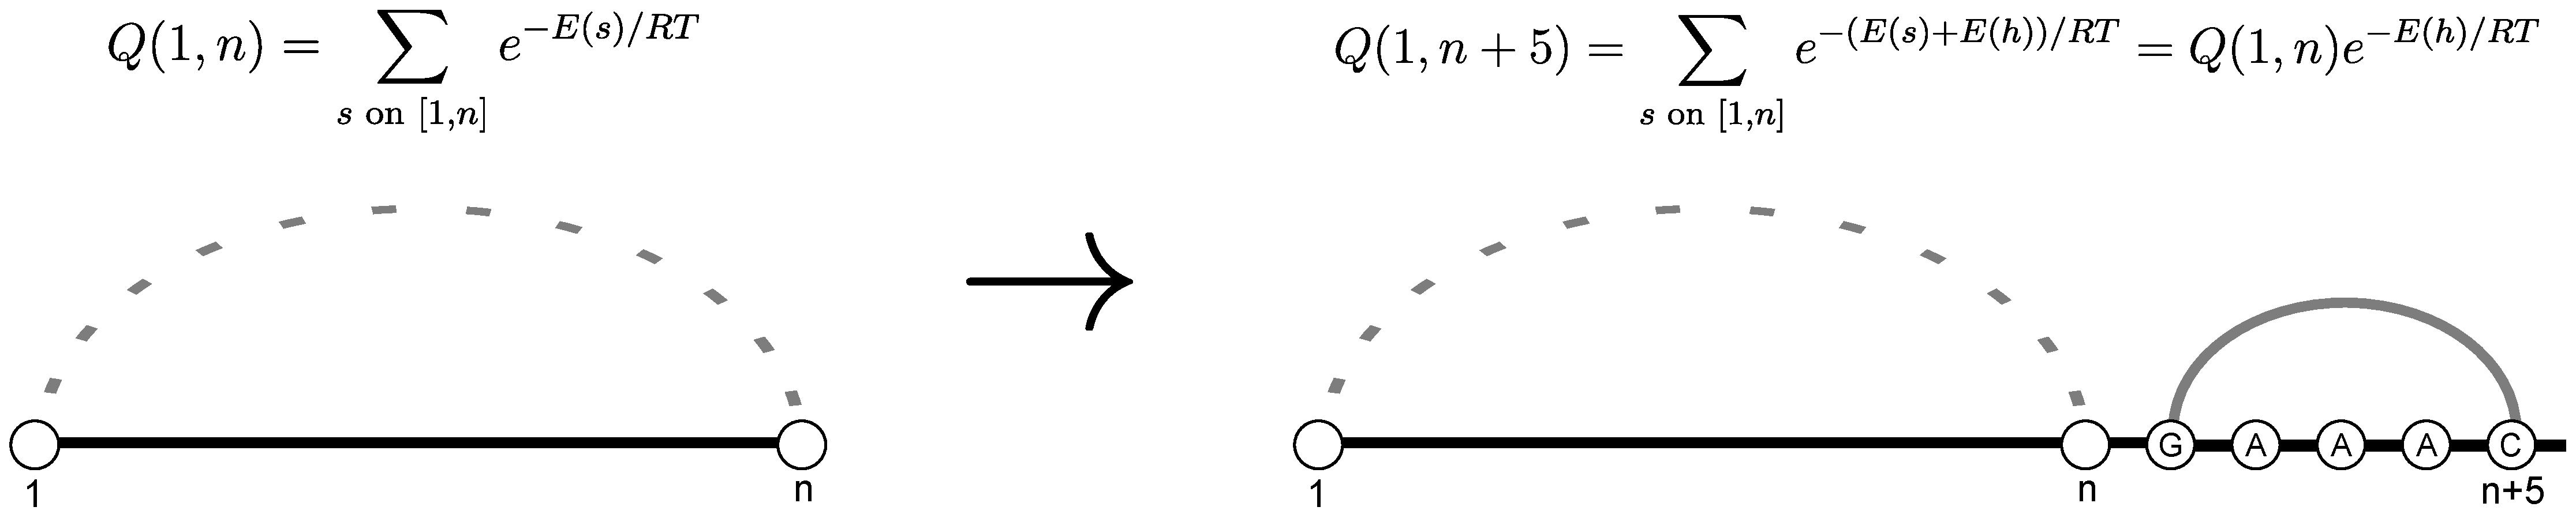
\includegraphics[width=\textwidth]{attachedHairpin.eps}
\caption{Extending the strand by adding an attached hairpin adds the
  energy of the hairpin to each structure. To compute the new
  partition function $Q(1, n+5)$, we do not need to sum the energies
  of all possible structures again, we can simply use the old value,
  $Q(1,n)$, and multiply it by the Boltzmann factor of the
  hairpin. This is the concept behind the dynamic programming
  algorithm.}
\label{fig:attachedHairpin}
\end{figure}
\begin{equation}
Q(1, n + 5) = \sum_{s \text{ on } [1,n]} e^{-(E(s) + E(h))/RT} = Q(1, n)e^{-E(h)/RT}. 
\end{equation}
This replaces an exponential-time computation (the sum), with a
constant time computation (multiplying the pre-computed $Q(1, n)$ with
the energy term). In general, this technique allows us to compute the
partition function efficiently, working up from $Q(1, 2)$ to
$Q(1,n)$. In computer science this technique is called dynamic
programming, a fancy name for the technique of storing the
results of a computation in a table for later use.

The dynamic programming algorithm for computing the partition function
of an RNA strands has several versions, depending on how in depth you
go with the energy model. The simplest algorithms allow for only
structures with nested base pairs. Nested means that the structure can
be represented with the parenthesis, for example
(((..((((....))))(((..)))..))), or without crossing pairs in expanded
loop diagrams such as the ones in Figure
\ref{fig:attachedHairpin}. Note that this kind of structure excludes
pseudoknots.  If you ignore psuedoknots, which is standard in the
field, and if you make an approximation that internal loops will never
exceed a certain length, the fastest algorithm runs in $O(n^3)$. We
believe that we can streamline this computation even more, taking
advantage of the fact that empirically, the number of probable base
pairs of a strand of length $n$ seems to grow like $n$, not
$n^2$. This is the same result we used to speed up the stochastic
traceback algorithm and potentially a partition function algorithm
that includes pseudoknots. The algorithm will be presented in its
simplest form, with more complicated versions available in the
appendices.

\section{Motivation}

In certain situations, such as partition function clustering, the
partition function is computed and recomputed several times. If the
partition function takes on the order of hours or days to compute,
this can make partition function clustering a bad option. However in
these situations it is also true that the partition function is
recomputed with almost the same properties, just certain pairs
restricted. This motivates a method of computing the partition
function using a known pairs heueristic to prune away unneccesary
computation.

This concept has already been implemented to great success in the
stochastic traceback algorithm. We've been able to show via experiment
that the partition function only admits roughly $O(n)$ pairs with
probabilities above thresholds around the machine precision limit. If
we have the partition function already computed, we can recompute it
by only adding in pairs that have sufficient probability. We can also
extend this method: if a good heuristic appears in the future, one
that can eliminate a large number of pairs, while being
computationally cheap, we should be able to use the results to speed
up the partition function computation.

\section{Computation}

The standard way of computing the partition function involves filling
out a table where the $(i,j)$ member represents the partition function
for the substrand from base $i$ to base $j$. Because the energy model
for RNA is (mostly) linear, the partition function from $i$ to $j$ can
be expressed as a function of nearby members of this table. This
function is the recurrence relation for the partition function of
RNA. Because the free energy model is so complicated and has gone
through many iterations, differenct RNA folding software packages
implement different versions of the recurrence relation, and they vary
widely in complexity.

The definitive representation of the recurrence relation for RNA was
formulated in 1990 by J.S. McCaskill in his landmark paper \emph{The
Equilibrium Partition Function and Base Pair Binding Probabilities for
RNA Secondary Structure} [TODO: cite?]. The formula is also presented
better and explained well by a later paper by Dirks and Pierce in 2003
(Dirks \& Peirce 2003). Starting at the outermost layer of this
relation, the formula for the partition function of the strand from
base $i$ to base $j$ is:

\begin{equation} Q(i,j) = 1 + \sum_{i \leq d < e \leq j}Q(i, d - 1)
Q^b(d, e) \end{equation}

The theory behind this formula is that the partition function is a sum
of the empty state (the first term, 1) and the state with at least 1
pair, the furthest pair to the right being pair $(d,e)$. The term
$Q^b(d,e)$ is the partition function assuming that base $d$ and base
$e$ are paired. This function has the following recursion relation:

\begin{equation} Q^b(i, j) = e^{-\frac{\text{Hairpin}(i,j)}{RT}} +
\sum_{i \leq d < e \leq j} e^{\frac{\text{Interior}(i, d, e,
j)}{RT}}Q^b(d,e) + \sum_{i \leq d < e \leq j} Q^m(i + 1, d - 1)Q^b(d,
e) e^{-\frac{\alpha_1 + 2\alpha_2 + \alpha_3(j-e-1)}{RT}}
\end{equation}

The theory behind this formula is that the partition function for a
strand assuming $i$ and $j$ are paired includes 3 cases:

\begin{enumerate}

\item

There are no bases paired between $i$ and $j$, the loop is a hairpin
and uses the energy function for a hairpin loop, we call
$\text{Hairpin}(i,j)$, which consists of data table lookups.

\item There is an internal loop between $i$ and $j$ and a second pair
$d$ and $e$. This uses a different energy model, we call
$\text{Internal}(i,j)$ and also consists of data table lookups.

\item There is a multiloop formed by the pair $i$ and $j$, which must
be carefully accounted for using a special model for multiloops.

\end{enumerate}

The multiloop partition function, $Q^m(i, j)$ is the last piece of the
puzzle. The formula is:

\begin{equation} Q^m(i, j) = \sum_{i \leq d < e \leq j}
e^{-\frac{\alpha_2 + \alpha_3(d-i) + \alpha_3(j-e)}{RT}} Q^b(d,e) +
Q^m(i, d - 1)Q^b(d, e) e^{-\frac{\alpha_2 + \alpha_3(j-e)}{RT}}
\end{equation}

In english, this just means we sum up all the ways to just have 1
pair, and then all the ways to have more than one pair. The case with
no pairs is not included, as in the original recursion in $Q^b$,
$Q^m(i+1, d-1)Q^b(d,e)$ must yield at least 2 pairs. Since $Q^b$ makes
one, then $Q^m$ must make at least 1.

For example, the UNAFold software package implements a particularly
hairy recurrence relation. Define $Q(i,j)$ as the partition function
from $i$ to $j$, $Q'(i,j)$ to be the partition function from $i$ to
$j$, assuming $i$ and $j$ are paired, and define $Q^1(i,j)$ to be the
partition function from $i$ to $j$, assuming exactly 1 pair happens on
that interval, and that pair happens with base $i$. The recurrence
relation is therefore

[recurrence relation]

Note the terms $Z_{ND}$, $Z_{3'D}$, $Z_{5'D}$, and $Z_{DD}$ are extra
free energy terms corresponding to 'dangle energies' which are the
results of an experiment later implemented in the model to improve it
from the standard energy model. In addition there are AU penalty terms
appended to where pairs are made, as AU and GU pairs have penalties
associated with forming. These additional energy terms improve the
model's predictive ability and bring the model closer to the "truth",
however it unfortunately makes the partition function seem very
threatening.

Our new partition function relation has the following theory behind
it: Assume we have the functions $I : B \to \{B\}$ and $J : B \to
\{B\}$ that return the set of all probably pairs for a base $i$ or a
base $j$, respectively. The recurrence relation can be reformulated in
the following way:

\section{Derivation of new Q(i, j) formula}

In UNAfold, we have that the old recurrence relations were as follows:

\begin{equation}
Q(i,j) = \sum_{k=i}^j \left ( Q(i, k-1) + e^{-\frac{b(k-i)}{RT}}  \right )Q^1(k, j)
\end{equation}
where 
\begin{equation}
\begin{split}
Q^1(i, j) = \ \ & Q^1(i, j - 1) e^{-\frac{b}{RT}}  \\
 +\ & e^{-\frac{c}{RT} }Z_{ND}(i, j) Q'(i, j)  \\
+\ & e^{-\frac{b + c}{RT}}Z_{5'D}(i + 1, j)Q'(i + 1, j)  \\
+\ &  e^{-\frac{b + c}{RT}}Z_{3'D}(i, j-1)Q'(i, j - 1)  \\
+\ &  e^{-\frac{2b + c}{RT}}Z_{DD}(i + 1, j-1)Q'(i + 1, j-1) 
\end{split}
\end{equation}
\noindent
We can expand the recursive definition of $Q^1(i,j)$:

\begin{equation}
\begin{split}
Q^1(i, j) = \sum_{k' = i + 1}^j e^{-\frac{b(j - k')}{RT} } \bigg [ \ 
  & e^{-\frac{c}{RT} }Z_{ND}(i, k') Q'(i, k') \\
 +\ & e^{-\frac{b + c}{RT}}Z_{5'D}(i + 1, k')Q'(i + 1, k') \\ 
+\  & e^{-\frac{b + c}{RT}}Z_{3'D}(i, k'-1)Q'(i, k' - 1) \\
+\  & e^{-\frac{2b + c}{RT}}Z_{DD}(i + 1, k'-1)Q'(i + 1, k'-1) \   \bigg ]
\end{split}
\end{equation}
\noindent
Plugging this into $Q(i,j)$ we get:

\begin{equation}
\begin{split}
Q(i, j) = \sum_{k= i}^j\ \sum_{k' = k + 1}^j \left (  Q(i, k-1) + e^{-\frac{b(k-i)}{RT}} \right ) e^{-\frac{b(j - k')}{RT} } \bigg [ \ 
  & e^{-\frac{c}{RT} }Z_{ND}(k, k') Q'(k, k')  \\
+\  & e^{-\frac{b + c}{RT}}Z_{5'D}(k + 1, k')Q'(k + 1, k') \\ 
+\ & e^{-\frac{b + c}{RT}}Z_{3'D}(k, k'-1)Q'(k, k' - 1) \\
+\  & e^{-\frac{2b + c}{RT}}Z_{DD}(k + 1, k'-1)Q'(k + 1, k'-1) \   \bigg ]
\end{split}
\end{equation}
\noindent
Now we'll take the $j$th element of the second sum and split it out (note that the $j$th part of the 1st sum has no elements to sum now, so we can decrement that too):
\begin{equation}
\begin{split}
Q(i, j) = \sum_{k= i}^{j-1}\ \sum_{k' = k + 1}^{j-1} \left (  Q(i, k-1) + e^{-\frac{b(k-i)}{RT}} \right ) e^{-\frac{b(j - k')}{RT} } \bigg [ \ 
  & e^{-\frac{c}{RT} }Z_{ND}(k, k') Q'(k, k')  \\
+ \  & e^{-\frac{b + c}{RT}}Z_{5'D}(k + 1, k')Q'(k + 1, k')\\ 
+\   & e^{-\frac{b + c}{RT}}Z_{3'D}(k, k'-1)Q'(k, k' - 1) \\
+\  & e^{-\frac{2b + c}{RT}}Z_{DD}(k + 1, k'-1)Q'(k + 1, k'-1) \   \bigg ] \\
+\ \sum_{k=i}^j  \left (  Q(i, k-1) + e^{-\frac{b(k-i)}{RT}} \right ) \bigg [ \ 
  & e^{-\frac{c}{RT} }Z_{ND}(k, j) Q'(k, j) \\
+\  & e^{-\frac{b + c}{RT}}Z_{5'D}(k + 1, j)Q'(k + 1, j) \\ 
+\  & e^{-\frac{b + c}{RT}}Z_{3'D}(k, j-1)Q'(k, j - 1) \\
 +\  & e^{-\frac{2b + c}{RT}}Z_{DD}(k + 1, j-1)Q'(k + 1, j-1) \   \bigg ]
\end{split}
\end{equation}
\noindent
Notice that the double sum is simply $Q(i,j-1)e^{-b/RT}$ and the terms of the second, single sum are over the pairs with $j$ or $j-1$. Therefore, we can use our heuristic for the pairs of $j$ and $j-1$ to produce the following computation for $Q(i, j)$ which is much more efficient than the previous ones:
\begin{equation}
\begin{split}
Q(i,j) = Q(i, j-1)e^{-b/RT} +  \sum_{k(j)} & \bigg [  \left (  Q(i, k-1) + e^{-\frac{b(k-i)}{RT}} \right ) \
   e^{-\frac{c}{RT} }Z_{ND}(k, j) Q'(k, j)  \\
+\ & \left (  Q(i, k-2) + e^{-\frac{b(k-i-1)}{RT}} \right )    e^{-\frac{b + c}{RT}}Z_{5'D}(k, j)Q'(k, j) \   \bigg ]  \\
+\  \sum_{l(j-1)} & \bigg [  \left (  Q(i, l-1) + e^{-\frac{b(l-i)}{RT}} \right ) \
   e^{-\frac{c}{RT} }Z_{ND}(l, j-1) Q'(l, j-1)  \\
+\ & \left (  Q(i, l-2) + e^{-\frac{b(l-i-1)}{RT}} \right )   e^{-\frac{2b + c}{RT}}Z_{DD}(l, j-1)Q'(l, j-1) \   \bigg ] 
\end{split}
\end{equation}

\section{Derivation of new Q'(i, j) formula}
For $Q'(i, j)$ we start with the recursion:

\begin{equation}
\begin{split}
Q'(i,j) = Z_H(i, j) &+ Z_S(i, j) Q'(i+1, j-1) + QBI(i, j) \\
+\ & e^{-\frac{a+c}{RT}}Z_{ND}(j, i) \sum_{k = i + 3}^{j-5}Q(i+1, k - 1)Q^1(k, j-1)  \\
+\ & e^{-\frac{a+b+c}{RT}}Z_{3'D}(j, i) \sum_{k = i + 4}^{j-5}Q(i+2, k - 1)Q^1(k, j-1)  \\
+\ & e^{-\frac{a+b+c}{RT}}Z_{5'D}(j, i) \sum_{k = i + 3}^{j-6}Q(i+1, k - 1)Q^1(k, j-2) \\
+\ & e^{-\frac{a+2b+c}{RT}}Z_{DD}(j, i) \sum_{k = i + 4}^{j-6}Q(i+2, k - 1)Q^1(k, j-2) 
\end{split}
\end{equation}
\noindent
The 4 for loops in this make this an expensive computation as the number of bases gets very high. However, these for loops are very similar to the partition function in structure. Indeed, we could perhaps replace each of them with a function of the form $Q^m(i, j)$ defined as

\begin{equation}
Q^m(i, j) = \sum_{k = i +3}^{j-5} Q(i + 1, k - 1) Q^1(k, j - 1)
\end{equation} 
\noindent
Which would simplify the previous sum to a constant time computation, provided we have memoized $Q^m$:
\begin{equation}
\begin{split}
Q'(i,j) = Z_H(i, j) &+ Z_S(i, j) Q'(i+1, j-1) + QBI(i, j)  \\
+\ & e^{-\frac{a+c}{RT}}Z_{ND}(j, i) Q^m(i, j)  \\
+\ & e^{-\frac{a+b+c}{RT}}Z_{3'D}(j, i) Q^m( i + 1, j) \\
+\ & e^{-\frac{a+b+c}{RT}}Z_{5'D}(j, i) Q^m(i, j- 1) \\
+\ & e^{-\frac{a+2b+c}{RT}}Z_{DD}(j, i) Q^m(i + 1, j -1)
\end{split}
\end{equation}

\noindent
Now there just needs to be a way to efficiently compute $Q^m$. First we substitute in the expanded version of $Q^1$:

\begin{equation}
\begin{split}
Q^m(i, j) = \sum_{k = i + 3}^{j - 5}\  \sum_{k' = k + 1}^{j- 1} Q(i + 1, k - 1)  e^{-\frac{b(j - k')}{RT} } \bigg [ \ 
  & e^{-\frac{c}{RT} }Z_{ND}(k, k') Q'(k, k') \\
+\  & e^{-\frac{b + c}{RT}}Z_{5'D}(k + 1, k')Q'(k + 1, k') \\ 
 +\ & e^{-\frac{b + c}{RT}}Z_{3'D}(k, k'-1)Q'(k, k' - 1) \\
+\  & e^{-\frac{2b + c}{RT}}Z_{DD}(k + 1, k'-1)Q'(k + 1, k'-1) \   \bigg ]
\end{split}
\end{equation}

\noindent
Then we do as before and seperate out the $j$th term of the second sum. Note that there seems to be an additional sum needed to account that I've decreased the first sum's endpoint to $j-6$, but the sum ends up being from $k'= j-4$ to $k' = j -2$ and since $Q'$ for bases less than 4 apart is 0 due to hairpin loop rules, this sum is equal to zero.
\begin{equation}
\begin{split}
Q^m(i, j) = \sum_{k = i + 3}^{j - 6}\  \sum_{k' = k + 1}^{j- 2} Q(i + 1, k - 1)  e^{-\frac{b(j - k'-1)}{RT} } \bigg [ \ 
  & e^{-\frac{c}{RT} }Z_{ND}(k, k') Q'(k, k') \\
+ \  & e^{-\frac{b + c}{RT}}Z_{5'D}(k + 1, k')Q'(k + 1, k') \\ 
+ \  & e^{-\frac{b + c}{RT}}Z_{3'D}(k, k'-1)Q'(k, k' - 1) \\
 + \  & e^{-\frac{2b + c}{RT}}Z_{DD}(k + 1, k'-1)Q'(k + 1, k'-1) \   \bigg ]\\
+ \ \sum_{k = i + 3}^{j - 5}\ Q(i + 1, k - 1)  \bigg [ \ 
  & e^{-\frac{c}{RT} }Z_{ND}(k, j-1) Q'(k, j-1)  \\
+ \  & e^{-\frac{b + c}{RT}}Z_{5'D}(k + 1, j-1)Q'(k + 1, j-1) \\ 
  + \ & e^{-\frac{b + c}{RT}}Z_{3'D}(k, j-2)Q'(k, j-2)\\
+ \  & e^{-\frac{2b + c}{RT}}Z_{DD}(k + 1, j-2)Q'(k + 1, j-2) \   \bigg ]\ 
\end{split}
\end{equation}
\noindent
The double sum is again going to be equal to $Q^m(i, j -1)e^{-b/RT}$, and the second sum can be made much more efficient by our heuristic. 
\begin{equation}
\begin{split}
Q^m(i, j) = Q^m(i, j - 1)e^{-b/RT} + \sum_{k(j - 1)} \bigg [ & Q(i + 1, k - 1)   
  e^{-\frac{c}{RT} }Z_{ND}(k, j-1) Q'(k, j-1)  \\
 + \ &Q(i + 1, k - 2) e^{-\frac{b + c}{RT}}Z_{5'D}(k, j-1)Q'(k, j-1)  \bigg ]\ \\
+ \sum_{k(j-2)} \bigg [ & Q(i + 1, k - 1)   
  e^{-\frac{c}{RT} }Z_{3'D}(k, j-2) Q'(k, j-2)  \\
  +\ &Q(i + 1, k - 2) e^{-\frac{b + c}{RT}}Z_{DD}(k, j-2)Q'(k, j-2)  \bigg ]
\end{split}
\end{equation}
\noindent

Since the $k$s for any individual $j$ are found to be quite limited, the final form should be much more efficient at computing the $Q'(i, j)$.

Note that for $Q$ and in many places for $Q'$, instead of a sum over
the known $k$ that could possibly begin a leftmost pair, we see a
double sum. One of them over $k$ that could end a leftmost pair, and
this sum is limited to a certain length below $j$. This is just making
the same assumption that the internal loop computation makes: there
are not arbitrarily long strands without base pairs, after a certain
number of bases it becomes overwhelmingly more likely to make a base
pair that we can virtually ignore the energy of the the cases of
length beyond a certain $L$.

As for the seocnd sum, since the number of probable pairs for a base
$i$ has been shown empirically to be roughly constant, regardless of
length, the second sum is essentially constant. What this all means is
that all $O(n^2)$ computations of $Q(i,j)$'s are roughly constant
time. This means that the overall algorithm is $O(n^2)$, an
improvement over the previous algorithms asymptotic bound by and order
of $n$!



\section{Results}

[TODO: include timing plots for new partition function]

Calculating the partition function is still difficult, but it can be
improved in the asymptotic case. The results show that the new
computation has a large constant factor in the beginning of the
algorithm. This could be related to the way the internal loop
partition function is calculated, where we still have an $O(n^3)$
algorithm until the number of nucleotides is greater than 30. This
effect is relatively diminished as we get into the 1000s in term of
base count, but it still is a large constant factor. As we increase
the probability barrier, we get further reductions in runtime.

[TODO: include plot with different times for different probability
thresholds]

A large part of the verification of an improved algorithm is showing
that it produces acceptable results compared to the old algorithm, as
you can see in the plot, our algorithm gives the same results up to 1
part in 1 million [TODO: check this]. Increasing the probability
threshold changes the results by [TODO: find out].

[TODO: include plot of verification]

\section{Conclusion}

The partition function computation is hard and is a limiting factor in
RNA structure prediction. However, given a heuristic to predict the
base pairs, we can make the algorithm run faster. These improvements
can be used in applications such as clustering based on our nestedness
measure, using the partition function. These improvements also open up
several possible branches for further investigation. Can a heuristic
be generated before the partition function is computed, so that the
pairs can be restricted and the computation done in much faster time
than the $O(n^3)$ algorithm? Could this concept be applied to the
pseudoknot algorithm to possibly speedup the computation for that as
well? Applications of this sort could have tremendous impact on RNA
secondary structure prediction, opening up incredible avenues of
potential.

